\documentclass{beamer}

\mode<presentation>
{
  \usetheme{default}      % or try Darmstadt, Madrid, Warsaw, ...
  \usecolortheme{default} % or try albatross, beaver, crane, ...
  \usefonttheme{default}  % or try serif, structurebold, ...
  \setbeamertemplate{navigation symbols}{}
  \setbeamertemplate{caption}[numbered]
} 

\usepackage[english]{babel}
\usepackage[utf8x]{inputenc}
\usepackage{graphicx} %Loading the package
\graphicspath{{figures/}} %Setting the graphicspath

%% --------------------------------------------
%% CSAFE customization
%% --------------------------------------------

\makeatletter
\usepackage{xpatch}
\patchcmd\beamer@@tmpl@frametitle{sep=0.3cm}{sep=1cm}{}{}
\makeatother

%% Define CSAFE colors
\definecolor{CSAFElightblue}{RGB}{35,168,224}
\definecolor{CSAFEblue}{RGB}{31,55,108}
\definecolor{CSAFEgreen}{RGB}{141,198,63}
\definecolor{CSAFEred}{RGB}{207,32,46} 
\definecolor{CSAFEgrey}{RGB}{128,130,133} 

%% Bullets and frame title colors
\setbeamercolor*{item}{fg=CSAFEgreen}
\setbeamercolor*{frametitle}{fg=white}

%% Title frame text color
\setbeamercolor*{title}{fg=white}
\setbeamercolor*{author}{fg=white}
\setbeamercolor*{date}{fg=white}
\setbeamercolor*{institute}{fg=white}



%% -End CSAFE customization



\title[Your Short Title]{Title of your presentation!}
\author{Your Name}
\institute{Your institution}
\date{The date of your talk}

\usepackage{Sweave}
\begin{document}
\input{CSAFE-template-concordance}
%\SweaveOpts{concordance=TRUE}
%\SweaveOpts{concordance=TRUE}

%% CSAFE Background
\usebackgroundtemplate{%
  
\includegraphics[width=\paperwidth,height=\paperheight]{csafe-cover-centered}} 


\begin{frame}
\vspace{-1.5cm}
%\hspace{6cm}
  \titlepage
\end{frame}

% Uncomment these lines for an automatically generated outline.
%\begin{frame}{Outline}
%  \tableofcontents
%\end{frame}


%% CSAFE Background
\usebackgroundtemplate{%
  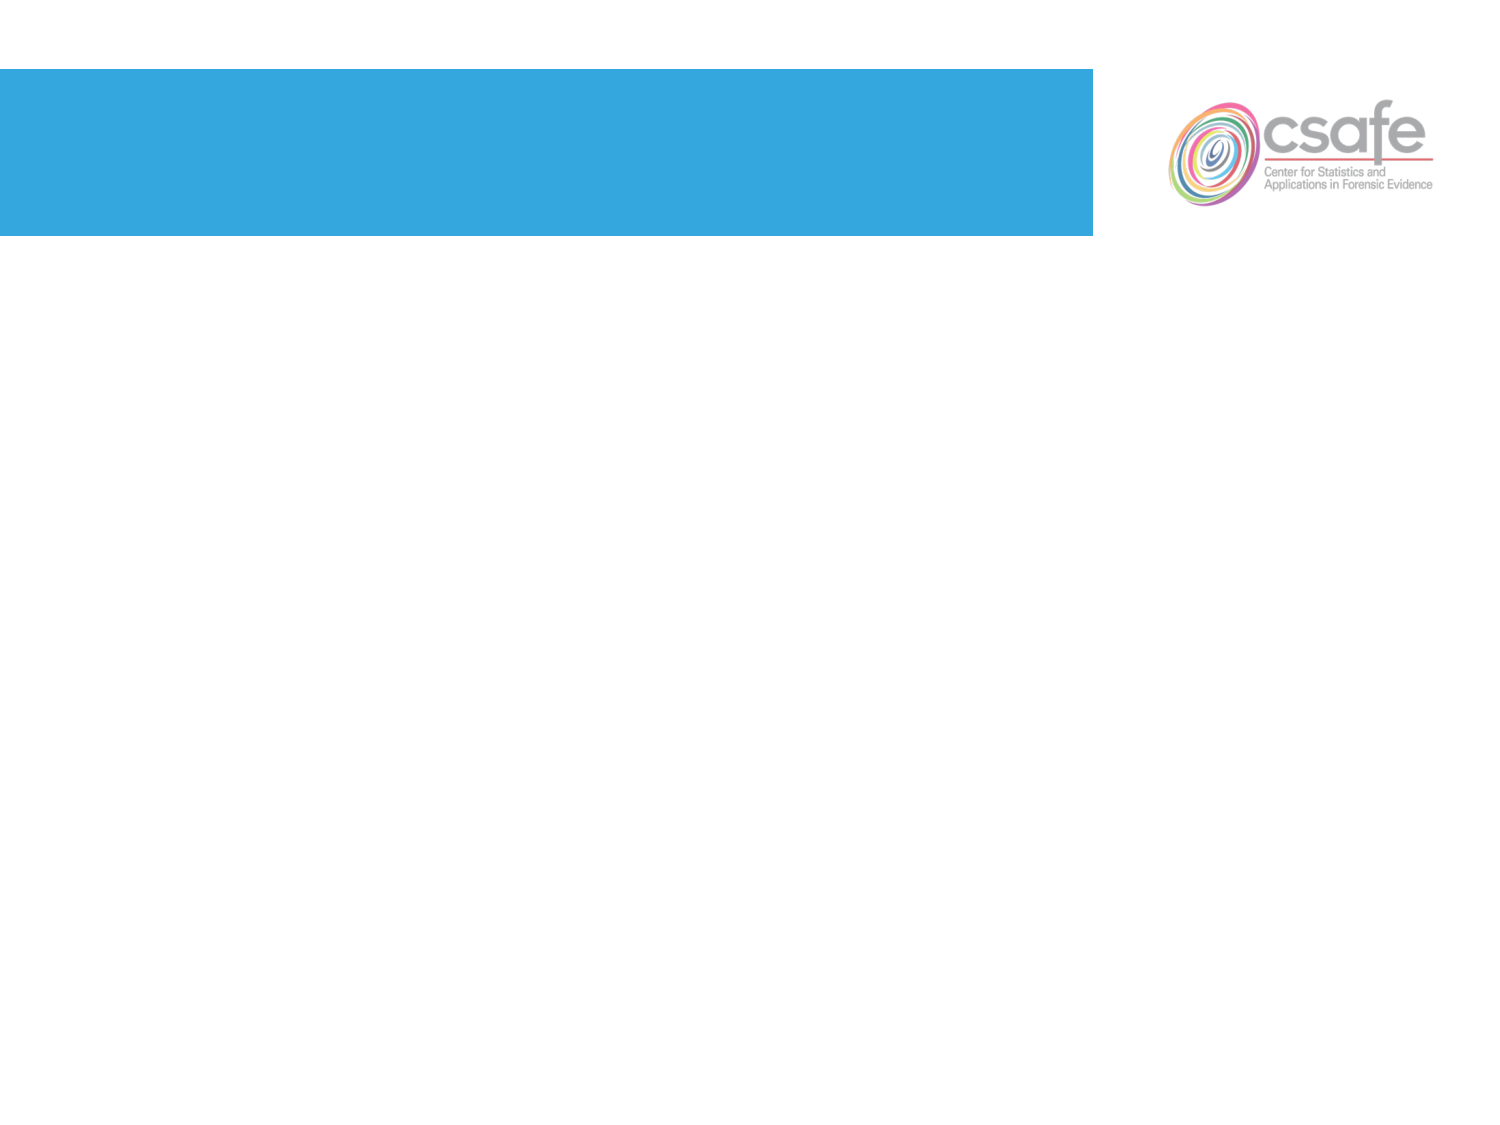
\includegraphics[width=\paperwidth,height=\paperheight]{csafe-blue-background}} 
 

\section{Introduction}



\begin{frame}[fragile]{Introduction}

\begin{itemize}
  \item Your introduction goes here!
  \item Use \texttt{itemize} to organize your main points.
\end{itemize}  


\begin{Schunk}
\begin{Sinput}
> a <- 2
\end{Sinput}
\end{Schunk}

`r a` 

\vskip 1cm

\begin{block}{Examples}
Some examples of commonly used commands and features are included, to help you get started.
\end{block}

\end{frame}

\section{Some \LaTeX{} Examples}

\subsection{Tables and Figures}

\begin{frame}{Tables and Figures}

\begin{itemize}
\item Use \texttt{tabular} for basic tables --- see Table~\ref{tab:widgets}, for example.
\item You can upload a figure (JPEG, PNG or PDF) using the files menu. 
\item To include it in your document, use the \texttt{includegraphics} command (see the comment below in the source code).
\end{itemize}

% Commands to include a figure:
%\begin{figure}
%\includegraphics[width=\textwidth]{your-figure's-file-name}
%\caption{\label{fig:your-figure}Caption goes here.}
%\end{figure}

\begin{table}
\centering
\begin{tabular}{l|r}
Item & Quantity \\\hline
Widgets & 42 \\
Gadgets & 13
\end{tabular}
\caption{\label{tab:widgets}An example table.}
\end{table}

\end{frame}

\subsection{Mathematics}

\begin{frame}{Readable Mathematics}

Let $X_1, X_2, \ldots, X_n$ be a sequence of independent and identically distributed random variables with $\text{E}[X_i] = \mu$ and $\text{Var}[X_i] = \sigma^2 < \infty$, and let
$$S_n = \frac{X_1 + X_2 + \cdots + X_n}{n}
      = \frac{1}{n}\sum_{i}^{n} X_i$$
denote their mean. Then as $n$ approaches infinity, the random variables $\sqrt{n}(S_n - \mu)$ converge in distribution to a normal $\mathcal{N}(0, \sigma^2)$.

\end{frame}

\end{document}
